% Copyright (c) 2015-2017, AIT Austrian Institute of Technology GmbH.
% REM All rights reserved. See file POWERFACTORY_FMU_LICENSE.txt for details.

\chapter{Exporting \pf models as FMUs}
\label{sec:export}

For the purpose of co-simulation, it is necessary to define a notion of time within the simulation model and to export this model in a way that allows to execute it.
For \pf there are several ways to do so, but in general the process involves 2 steps:
\begin{enumerate}

   \item \textbf{\pf models have to be created in a specific way}, which allows them to be used with the \fmipp \pf FMU export utility.
   
   \item These models are then \textbf{packaged as FMUs for Co-Simulation} with the help of the \fmipp \pf Export Utility.
   This can be either done by using a \textbf{graphical user interface} (see Figure~\ref{fig:gui_create}) or by executing a \textbf{Python script} from the command line.

\end{enumerate}
The following chapter explains the possible ways to do this.
Examples for all cases are given in Chapter~\ref{sec:examples}.

\begin{figure}[h!]
%\vspace*{1em}
\centering{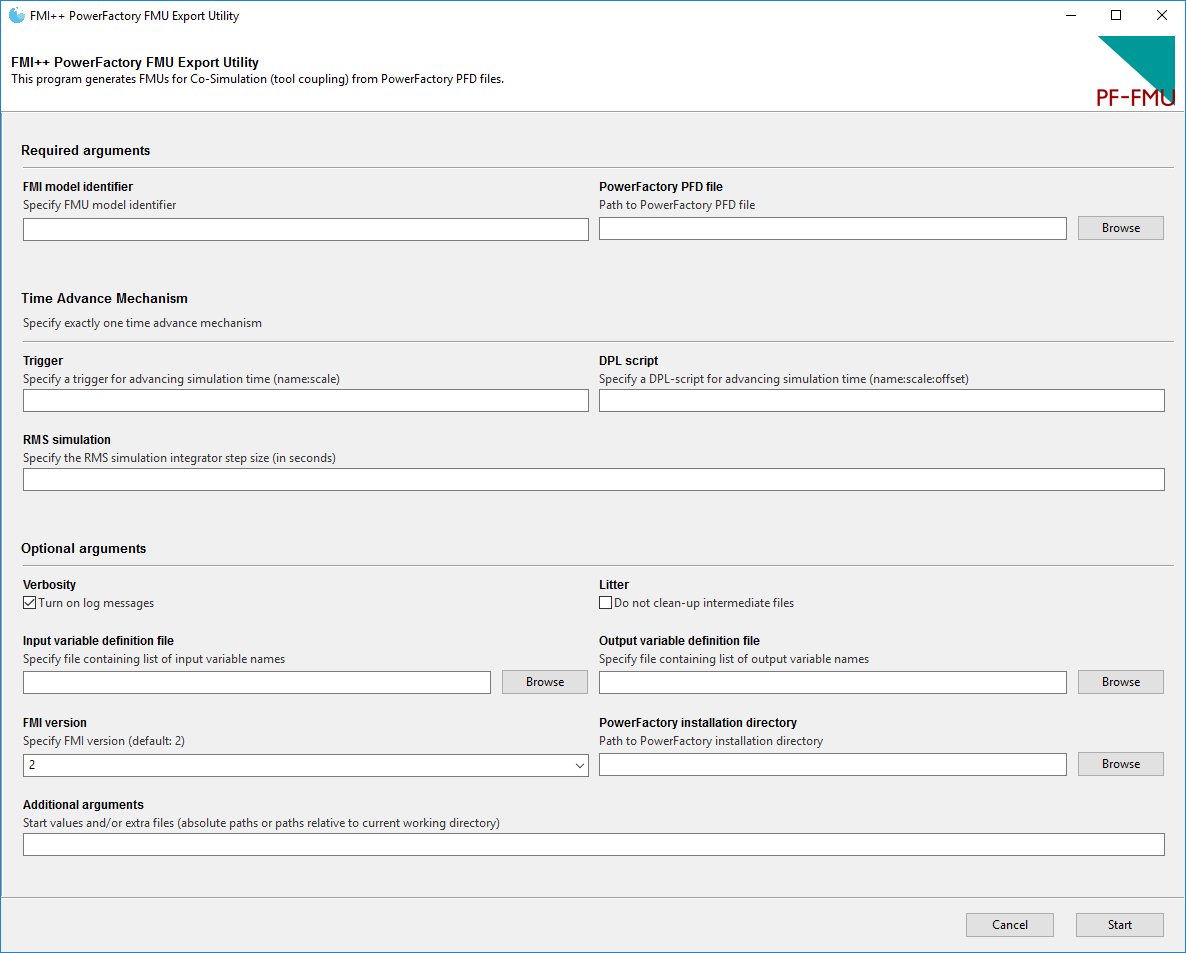
\includegraphics[width=\textwidth]{gui_create}}
\vspace*{-2mm}
\caption{Graphical user interface for creating FMUs for Co-Simulation from \pf models.}
\label{fig:gui_create}
\end{figure}

\section{Models using external time series and triggers}

\subsection{Creating models using external time series and triggers}

The method explained in this section can be used for creating models for quasi-static steady-state simulations.
It relies on \pf's functionality to associate object parameters with a time series by providing an external file, called a \emph{Parameter Characteristic from File} (type \texttt{ChaVecFile}).
The actual value of the parameter can be changed by associating a user-defined \emph{Trigger and Unit for File} (type \texttt{TriFile}) to such a time series.
Figure~\ref{fig:characteristics_from_file} shows the setup window for such a characteristic from file, which defines the associated external file (called \texttt{TestTriggers-characteristics.csv}) and the trigger (defined via the \texttt{Scale} field).
Figure~\ref{fig:trigger_for_file} shows the setup for the trigger itself.
\begin{figure}[h!]
%\vspace*{1em}
\centering{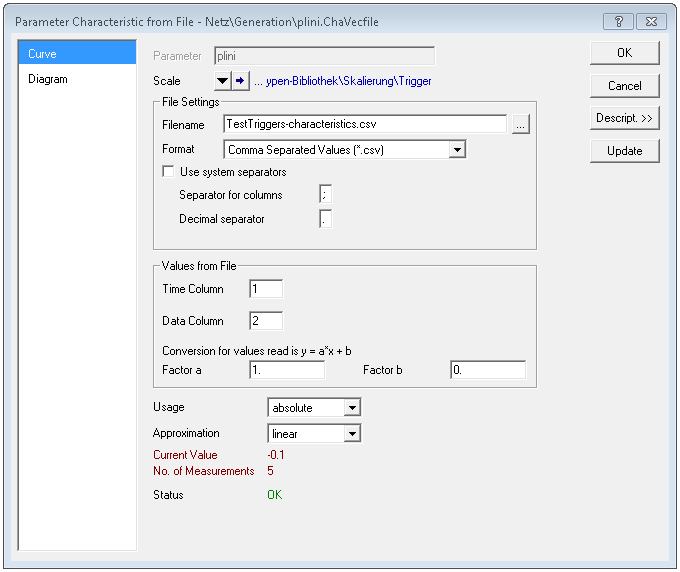
\includegraphics[width=0.9\textwidth]{characteristics_from_file}}
\vspace*{-2mm}
\caption{\pf window for defining a parameter characteristic from file.}
\label{fig:characteristics_from_file}
\vspace*{1em}
\centering{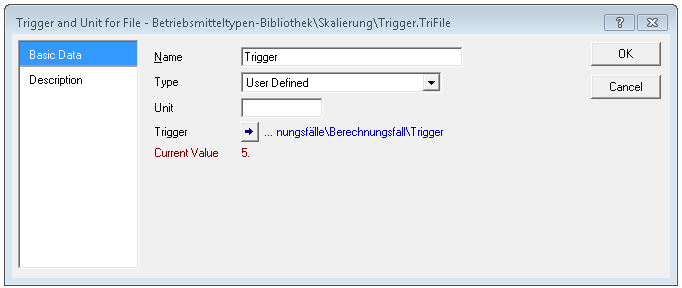
\includegraphics[width=0.85\textwidth]{trigger_for_file}}
\vspace*{-2mm}
\caption{\pf window for defining a trigger and unit for file.}
\label{fig:trigger_for_file}
\end{figure}

%\clearpage

To associate such a time series to a parameter do the following:
\begin{itemize}
  \item select the associated object (double-click)
  \item right-click the input field of the corresponding parameter to bring up the context menu
  \item first select \emph{Add Project Characteristic}, then \emph{Characteristic from File...}
  \item choose the previously created characteristic in the project browser
\end{itemize} 
Figure~\ref{fig:add_characteristics_from_file} shows how the context menus looks like for the example of associating a characteristic from file to the active power parameter of a general load.

\begin{figure}[h!]
\vspace*{2em}
\centering{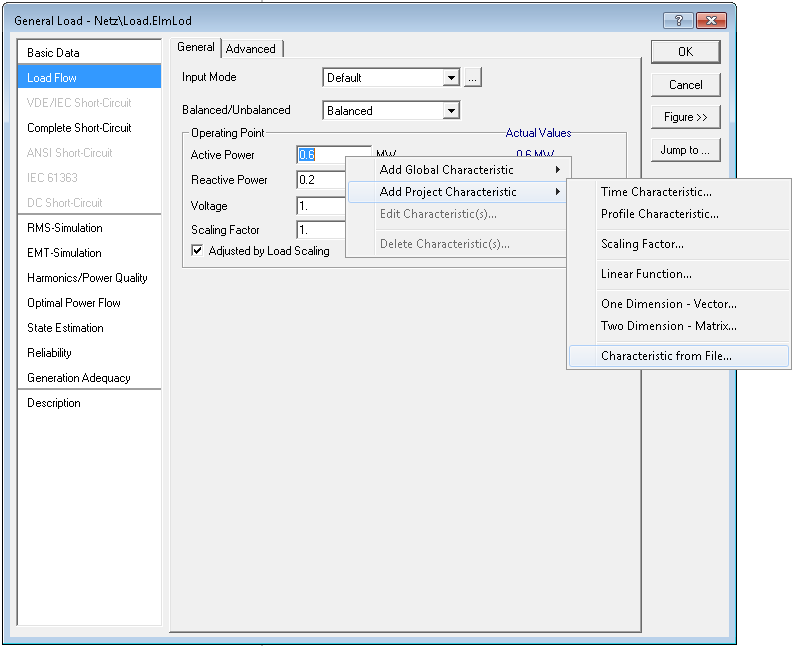
\includegraphics[width=0.9\textwidth]{add_characteristics_from_file}}
\caption{Context menus for associating a time series to a parameter.}
\label{fig:add_characteristics_from_file}
\end{figure}

\clearpage

\subsection{Exporting an FMU from a model using external time series and triggers}

\subsubsection*{Using the graphical user interface}

Once a \pf model according to the instructions above has been created, an FMU can be created with the help of the graphical user interface.
Switch to the installation directory and start program \texttt{powerfactory\_fmu\_install.exe} (double-click).
This should bring up the window shown in Figure~\ref{fig:gui_create}, where you can provide the following inputs:

\textit{Required arguments}:
\begin{itemize}
   \item \textbf{FMI model identifier}: Specify the FMU model identifier. 
   \emph{Attention}: The FMU model identifier must fulfill the restrictions for C function names!
   \item \textbf{\pf PFD file:} Export the \pf model as PFD file and provide its path (absolute or relative).
\end{itemize}

\textit{Time Advance Mechanism}:
\begin{itemize}
   \item \textbf{Trigger}:
   Triggers for simulation time advance need to be defined in the form \texttt{<name>:<scale>}.
   The \texttt{name} has to be given according to the trigger's object name in the PFD file.
   Times given to the FMU are interpreted as seconds, therefore the \texttt{scale} can be adjusted to match the trigger's internal unit of time (e.g., 60 for minutes or 3600 for hours).
   \item Leave the other boxes in this section empty.
\end{itemize}

\textit{Optional arguments}:
\begin{itemize}
   \item \textbf{Verbosity}: Turn on log messages.
   \item \textbf{Litter}: Do not clean-up intermediate files (e.g., log file with debug messages from Visual Studio compiler).
   \ietm \textbf{Input variable definition file} and \textbf{Output variable definition file}:
   Define which model variables of the \pf model should be exposed as input and output variables of the FMU.
   To do so, provide files containing lists of these variable names.
   These lists are expected to be in clear text, listing exactly one valid variable name per line.
   As explained in Section~\ref{sec:naming_convention:obj_param}, variable names are supposed to be of the  form \texttt{<obj-type>.<obj-name>.<param-name>}.
   \item \textbf{FMI version}: Specify FMI version (default: 2).
   \item \textbf{\pf installation directory}: Absolute path to \pf installation directory.\footnote{It is usually not necessary to provide the path to the \pf installation directory, unless the FMU is intended to run on another machine with a different installation directory path.}
   \item \textbf{Additional arguments}:
   \begin{itemize}
      \item Additional files may be specified (e.g., weather data or input/output name lists) that will be automatically copied to the FMU. The specified files paths may be absolute or relative.
      \item Start values for variables may be defined. For instance, to set variable with name \verb!var1! to value 12.34, specify \verb!var1=12.34! as optional argument.
   \end{itemize}
\end{itemize}


\subsubsection*{Export via Python script}

Alternatively, a \python script can be executed from the command prompt window (please refer to the \href{https://docs.python.org/3/faq/windows.html}{\python~FAQ} in case you need assistance with this).
Open the command prompt window and execute the script \texttt{powerfactory\_fmu\_create.py}:

\begin{verbatim}
python.exe <path_to_pf_fmu_dir>powerfactory_fmu_create.py [-h] [-v]
  [-f {1|2}] -m model_id -p pfd_file -i input_var_file -o output_var_file
  -t name:scale] [-d pf_install_dir] [additional_file_1 ... ]
  [var1=start_val1 ...]
\end{verbatim}

The path to the \fmipp \pf FMU export utility directory \verb!<path_to_pf_fmu_dir>! may be relative or absolute.
Optional arguments are enclosed by squared brackets \verb![!$\,$\ldots\verb!]!.
  
\textit{Mandatory input arguments}:
\begin{itemize}
  \item \verb!-m, --model-id!: specify FMU model identifier
  \item \verb!-p, --pfd-file!: path to PowerFactory PFD file
  \item \verb!-i, --input-var-file!: specify file containing list of input variable names
  \item \verb!-o, --output-var-file!: specify file containing list of output variable names
  \item \verb!-t, --trigger!: specify a trigger for advancing simulation time
\end{itemize}
\textit{Optional input arguments}:
\begin{itemize}
  \item \verb!-f, --fmi-version!: specify the FMI version (1: FMI~1.0, 2: FMI~2.0, default: 2)
  \item \verb!-v, --verbose!: turn on log messages
  \item \verb!-h, --help!: display the help screen
  \item \verb!-l, --litter!: do not clean-up intermediate files
  \item \verb!-d, --pf-install-dir!: path to \pf installation directory\footnote{It is usually not necessary to provide the path to the \pf installation directory, unless the FMU is intended to run on another machine with a different installation directory path.}
\end{itemize}
Files containing lists of input and output variable names are expected to be in clear text, listing exactly one valid variable name per line.
As explained in Section~\ref{sec:naming_convention:obj_param}, variable names are supposed to be of the  form \texttt{<obj-type>.<obj-name>.<param-name>}.

Triggers for simulation time advance need to be defined in the form \texttt{<name>:<scale>}.
The \texttt{name} has to be given according to the trigger's object name in the PFD file.
Times given to the FMU are interpreted as seconds, therefore the \texttt{scale} can be adjusted to match the trigger's internal unit of time (e.g., 60 for minutes or 3600 for hours).
Multiple triggers may be defined.

Additional files may be specified (e.g., CSV load profiles) that will be automatically copied to the FMU. The specified files paths may be absolute or relative.

Furthermore, start values for variables may be defined. For instance, to set a variable with the name \texttt{ElmLod.TestLoad.plini} to a value of 12.34, specify \texttt{ElmLod.TestLoad.plini=12.34} in the command line as optional argument.

Section~\ref{sec:examples:triggers} gives a concrete example of how to export such a model using time series and triggers as an FMU.

\newpage

\section{Models using a \dplscript to define the time}

\subsection{Creating models using a \dplscript to define the time}
\label{sec:export:create_model_dplscript}

The method explained in this section can be used for creating models for quasi-static steady-state simulations.
It relies on \pf's functionality to associate object parameters to 1-dimensional vectors, called \emph{Characteristic -- Vector} (type \texttt{ChaVec}).
The actual value of the parameter can be changed by associating the elements of such a vector to a \emph{Time Scale} (type \texttt{TriTime}) that maps each element to a specific point in time.
Time itself within the model can then be set with the help of a dedicated \dplscript.
Figure~\ref{fig:characteristics_from_vector} shows the setup window for such a vector characteristic, which defines the mapping of the values to the points in time defined by the time scale (defined via the \texttt{Scale} field).
Figure~\ref{fig:trigger_for_vector} shows the setup for the time scale itself.


\begin{figure}[h!]
\vspace*{1ex}
\centering{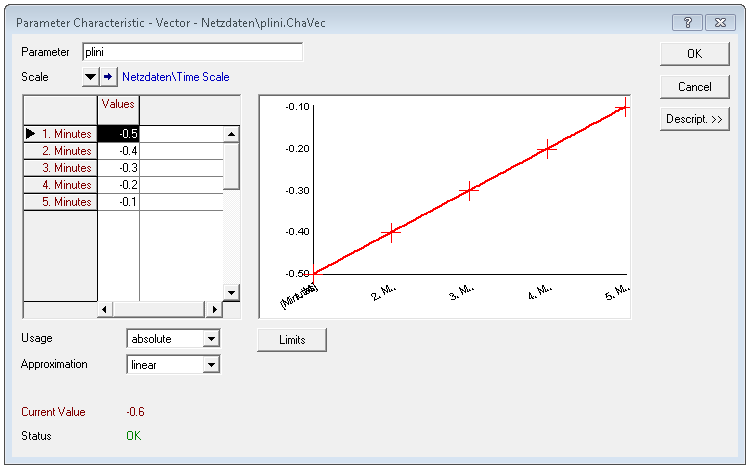
\includegraphics[width=0.9\textwidth]{characteristics_from_vector}}
\caption{\pf window for defining a parameter characteristic from a vector.}
\label{fig:characteristics_from_vector}
\end{figure}

\begin{figure}[h!]
\vspace*{1ex}
\centering{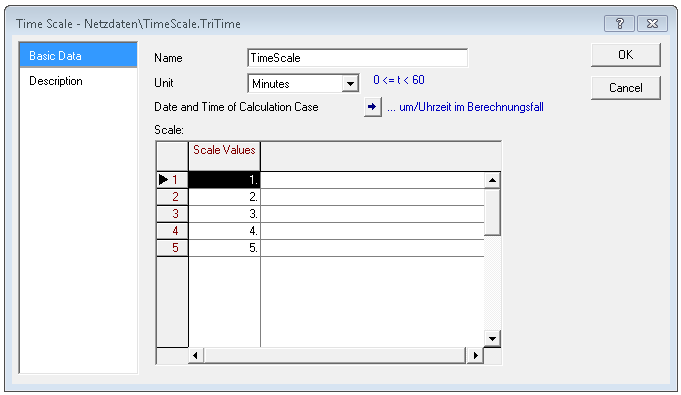
\includegraphics[width=0.85\textwidth]{trigger_for_vector}}
\caption{\pf window for defining a trigger and unit for a vector.}
\label{fig:trigger_for_vector}
\end{figure}

To associate such a vector characteristic to a parameter do the following:
\begin{itemize}
  \item select the associated object (double-click)
  \item right-click the input field of the corresponding parameter to bring up the context menu
  \item first select \emph{Add Project Characteristic}, then \emph{One Dimension -- Vector...}
  \item choose the previously created vector characteristic in the project browser
\end{itemize} 
Figure~\ref{fig:add_characteristic_vector} shows how the context menus looks like for the example of associating a characteristic from file to the active power parameter of a general load.

\begin{figure}[h!]
\vspace*{2em}
\centering{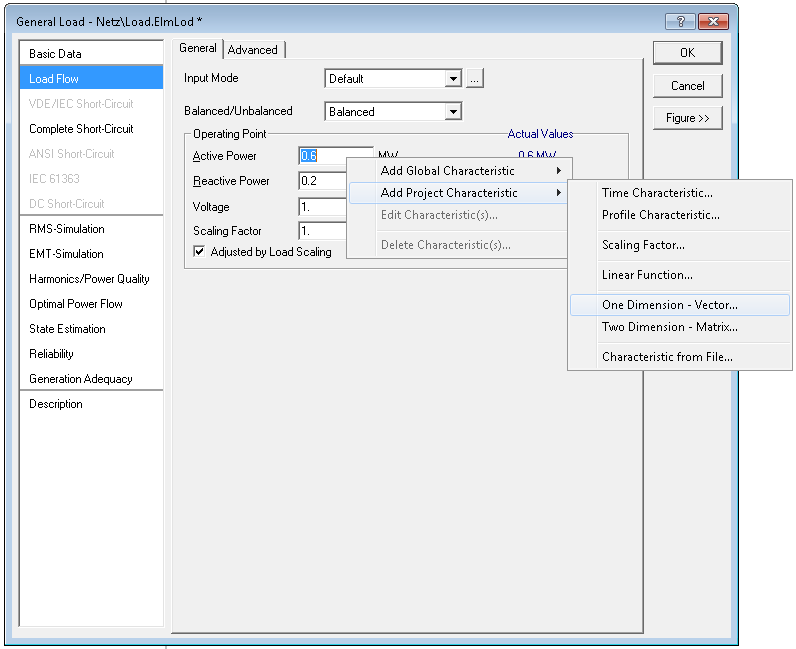
\includegraphics[width=0.9\textwidth]{add_characteristic_vector}}
\caption{Context menus for associating a vector characteristic to a parameter.}
\label{fig:add_characteristic_vector}
\end{figure}

\clearpage

In addition, the \dplscript for setting the time has to be provided.
Such a script could be of the following form:

\begin{Verbatim}[frame=single,commandchars=\\\{\}]

  \codeHighlightGreen{! Change date/time of active study case,}
  \codeHighlightGreen{! using the second of the year as input.}
  \codeHighlightGreen{!}
  \codeHighlightGreen{! ATTENTION: The script doesn't properly}
  \codeHighlightGreen{! handle simulation runs longer than one}
  \codeHighlightGreen{! year.}

  \codeHighlightBlue{object} \textcolor{black}{set_time;}

  \textcolor{black}{set_time =} \codeHighlightBlue{GetCaseObject}\textcolor{black}{(} \codeHighlightRed{'SetTime'} \textcolor{black}{);}

  \codeHighlightBlue{if} \textcolor{black}{( set_time ) \{}
  \textcolor{black}{  set_time:min = 0.0;}
  \textcolor{black}{  set_time:sec = 0.0;}
  \textcolor{black}{  set_time.SetTime( second_of_year * }\codeHighlightDarkRed{0.000277778}\textcolor{black}{ );}
  \textcolor{black}{\}}

\end{Verbatim}
The script's input is the second of the year, represented by variable \texttt{second\_of\_year} (compare to \dplscript setup in Figure~\ref{fig:dpl_script_setup})
The script calculates the hour of the year (by multiplication of $0.000277778 = 1 / 3600$) and and uses this value to set the model's time with the help of function \texttt{SetTime}.
\begin{figure}[h!]
\vspace*{1ex}
\centering{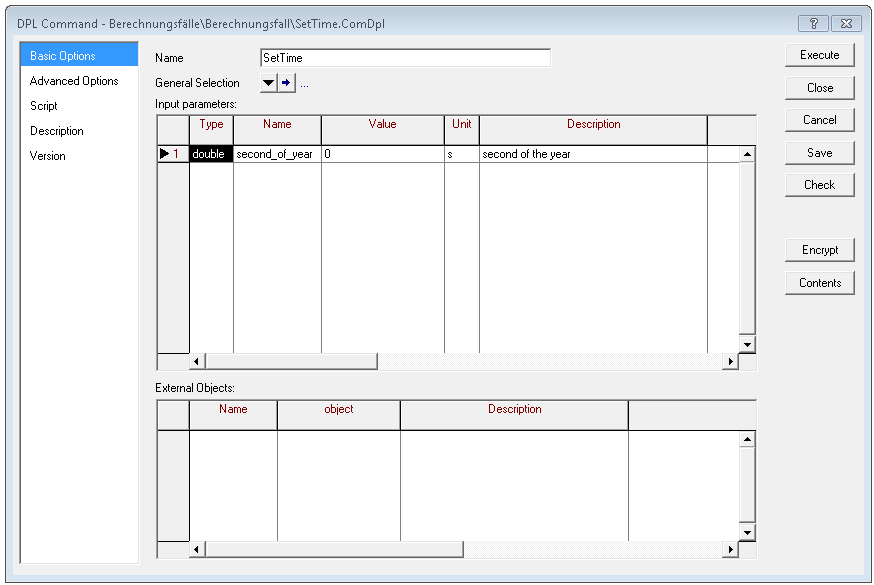
\includegraphics[width=0.95\textwidth]{dpl_script_setup}}
\vspace{-2mm}
\caption{\pf window for \dplscript setup.}
\label{fig:dpl_script_setup}
\end{figure}

\subsection{Exporting an FMU from a model using a \dplscript to define the time}

\subsubsection*{Using the graphical user interface}

Once a \pf model according to the instructions above has been created, an FMU can be created with the help of the graphical user interface.
Switch to the installation directory and start program \texttt{powerfactory\_fmu\_install.exe} (double-click).
This should bring up the window shown in Figure~\ref{fig:gui_create}, where you can provide the following inputs:

\textit{Required arguments}:
\begin{itemize}
   \item \textbf{FMI model identifier}: Specify the FMU model identifier. 
   \emph{Attention}: The FMU model identifier must fulfill the restrictions for C function names!
   \item \textbf{\pf PFD file:} Export the \pf model as PFD file and provide its path (absolute or relative).
\end{itemize}

\textit{Time Advance Mechanism}:
\begin{itemize}
   \item \textbf{DPL script}:
   Specify a DPL-script for advancing simulation time. 
   A single \dplscript may be specified to advance simulation time in the form \texttt{<name>:<scale>:<offset>}.
   The \texttt{name} has to be given according to the script's name in the PFD file.
   Times given to the FMU are interpreted as seconds, therefore the \texttt{scale} and \texttt{offset} can be adjusted to match the \dplscript's internal representation of time (e.g., 60 for minutes or 3600 for hours).
   \item Leave the other boxes in this section empty.
\end{itemize}

\textit{Optional arguments}:
\begin{itemize}
   \item \textbf{Verbosity}: Turn on log messages.
   \item \textbf{Litter}: Do not clean-up intermediate files (e.g., log file with debug messages from Visual Studio compiler).
   \ietm \textbf{Input variable definition file} and \textbf{Output variable definition file}:
   Define which model variables of the \pf model should be exposed as input and output variables of the FMU.
   To do so, provide files containing lists of these variable names.
   These lists are expected to be in clear text, listing exactly one valid variable name per line.
   As explained in Section~\ref{sec:naming_convention:obj_param}, variable names are supposed to be of the  form \texttt{<obj-type>.<obj-name>.<param-name>}.
   \item \textbf{FMI version}: Specify FMI version (default: 2).
   \item \textbf{\pf installation directory}: Absolute path to \pf installation directory.\footnote{It is usually not necessary to provide the path to the \pf installation directory, unless the FMU is intended to run on another machine with a different installation directory path.}
   \item \textbf{Additional arguments}:
   \begin{itemize}
      \item Additional files may be specified (e.g., weather data or input/output name lists) that will be automatically copied to the FMU. The specified files paths may be absolute or relative.
      \item Start values for variables may be defined. For instance, to set variable with name \verb!var1! to value 12.34, specify \verb!var1=12.34! as optional argument.
   \end{itemize}
\end{itemize}

\clearpage

\subsubsection*{Export via Python script}

Alternatively, a \python script can be executed from the command prompt window (please refer to the \href{https://docs.python.org/3/faq/windows.html}{\python~FAQ} in case you need assistance with this).
Open the command prompt window and execute the script \texttt{powerfactory\_fmu\_create.py}:

\begin{verbatim}
python.exe <path_to_pf_fmu_dir>powerfactory_fmu_create.py [-h] [-v] 
  [-f {1|2}] -m model_id -p pfd_file  -i input_var_file 
  -o output_var_file -s name:scale:offset [-d pf_install_dir] 
  [additional_file_1 ... ] [var1=start_val1 ...]
\end{verbatim}

The path to the \fmipp \pf FMU export utility directory \verb!<path_to_pf_fmu_dir>! may be relative or absolute.
Optional arguments are enclosed by squared brackets \verb![!$\,$\ldots\verb!]!.
  
\textit{Mandatory input arguments}:
\begin{itemize}
  \item \verb!-m, --model-id!: specify FMU model identifier
  \item \verb!-p, --pfd-file!: path to PowerFactory PFD file
  \item \verb!-i, --input-var-file!: specify file containing list of input variable names
  \item \verb!-o, --output-var-file!: specify file containing list of output variable names
  \item \verb!-s, --dpl-script!: specify a \dplscript for advancing simulation time
\end{itemize}
\textit{Optional input arguments}:
\begin{itemize}
  \item \verb!-f, --fmi-version!: specify the FMI version (1: FMI~1.0, 2: FMI~2.0, default: 2)
  \item \verb!-h, --help!: display the help screen
  \item \verb!-v, --verbose!: turn on log messages
  \item \verb!-l, --litter!: do not clean-up intermediate files
  \item \verb!-d, --pf-install-dir!: path to \pf installation directory\footnote{It is usually not necessary to provide the path to the \pf installation directory, unless the FMU is intended to run on another machine with a different installation directory path.}
\end{itemize}
Files containing lists of input and output variable names are expected to be in clear text, listing exactly one valid variable name per line.
As explained in Section~\ref{sec:naming_convention:obj_param}, variable names are supposed to be of the form \texttt{<obj-type>.<obj-name>.<param-name>}.

A single \dplscript may be specified to advance simulation time in the form \texttt{<name>:<scale>:<offset>}.
The \texttt{name} has to be given according to the script's name in the PFD file.
Times given to the FMU are interpreted as seconds, therefore the \texttt{scale} and \texttt{offset} can be adjusted to match the \dplscript's internal representation of time (e.g., 60 for minutes or 3600 for hours).

Additional files may be specified that will be automatically copied to the FMU. The specified files paths may be absolute or relative.

Furthermore, start values for variables may be defined. For instance, to set a variable with the name \texttt{ElmLod.TestLoad.plini} to a value of 12.34, specify \texttt{ElmLod.TestLoad.plini=12.34} in the command line as optional argument.

Section~\ref{sec:examples:dplscript} gives a concrete example of how to export such a model using a \dplscript as an FMU.


\newpage


\section{Models for RMS simulations}

\subsection{Creating models for RMS simulation}
\label{sec:export:create_model_rms}

The method explained in this section can be used for creating models for RMS simulations.

\subsubsection*{Sending simulation events as inputs}

This approach relies on \pf's functionality to associate objects with user-defined {\dslmodel}s via a composite model (type \texttt{ElmComp}).
By sending a so-called \emph{parameter event} (type \texttt{EvtParam}) to such a \dslmodel, the model's input parameters can be changed.
This change of input parameters can be easily propagated to the parameters of any object by connecting the \dslmodel with the corresponding object in a composite model.

\subsubsection*{Setup of \dslmodel FMIAdapter}

For sending events to a composite model, a dedicated compiled \dslmodel called \emph{FMIAdapter} is provided.
To include this \dslmodel into a \pf model, create a new empty \dslmodel (see \pf User Manual, Section~28.12.3 Defining DSL Models) and choose \emph{Compiled model}  as \emph{Model type}.
Then type \emph{fmiadapter.dll} into the field \emph{DLL-file}.\footnote{
  This works only if during the installation of the FMU export utility the DLL-file \emph{fmiadapter.dll} was successfully copied to the \pf installation directory.
  If this is not the case, it is also possible to select this file from the \emph{binaries} folder located in the installation directory of the FMU export utility. To do so, click on the button with the three dots.}
The resulting model definition should look like Figure~\ref{fig:fmiadapter_model_definition}.
It is recommended -- but not necessary -- to name this new \dslmodel as \emph{FMIAdapter} and store it in the project folder \emph{Library} $\to$ \emph{User Defined Models}.

\subsubsection*{Including \dslmodel FMIAdapter into a composite model}

To use the \dslmodel FMIAdapter, it has to be included into a composite model.
This can be done by simply adding a dedicated slot to a composite frame (see \pf User Manual, Section~28.10.2 The Composite Frame), see for instance Figure~\ref{fig:fmiadapter_slot}.
The corresponding slot does not have to be connected to any other slot.
FMIAdapter's output signal called \emph{trigger} is mostly intended for debugging purposes, sending a trigger signal whenever an event has been issued.

Figure~\ref{fig:fmiadapterconfig_composite_frame} shows an example of a composite frame that includes a dedicated FMIAdapter slot.
To send an event to a controller model (represented by slot \emph{Controller}), the corresponding simulation event definition (according to the naming convention in Section~\ref{sec:naming_convention:sim_evt}) would have to refer to the name of this specific slot and a parameter of the model associated to it.
See Section~\ref{sec:examples:rmssim} for more details on this example.

\subsubsection*{Retrieving outputs}

For retrieving outputs from an RMS simulation, object parameters can be accessed directly (just like in the case of quasi-static steady-state simulations).


\begin{figure}[h!]
\vspace*{1em}
\centering{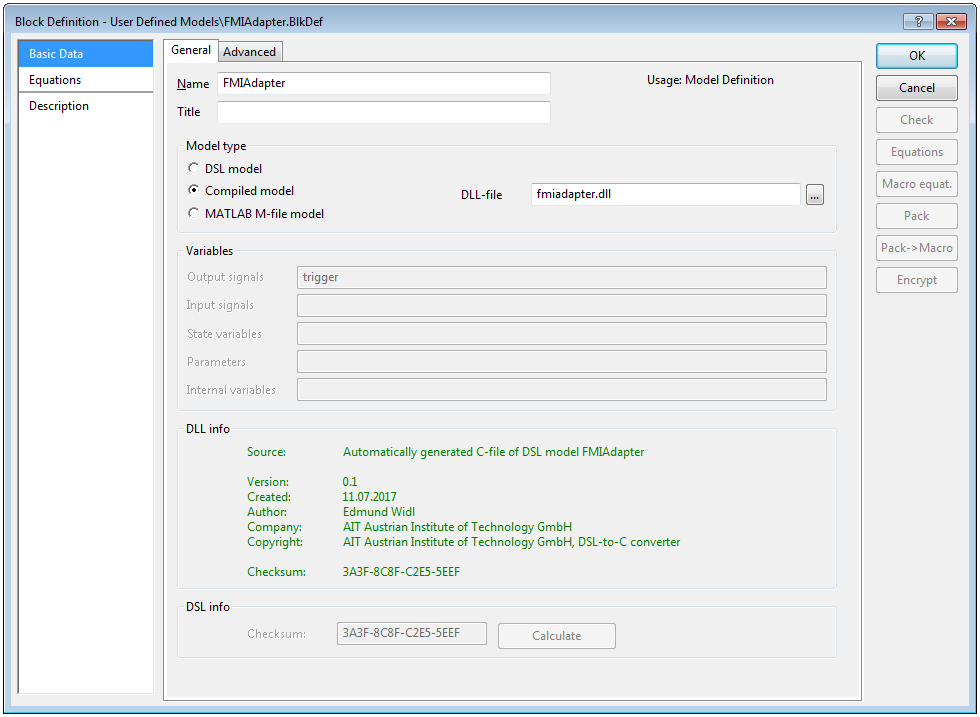
\includegraphics[width=0.98\textwidth]{fmiadapter_model_definition}}
\caption{Block definition of compiled \dslmodel FMIAdapter.}
\label{fig:fmiadapter_model_definition}
\end{figure}

\begin{figure}[h!]
\vspace*{1em}
\centering{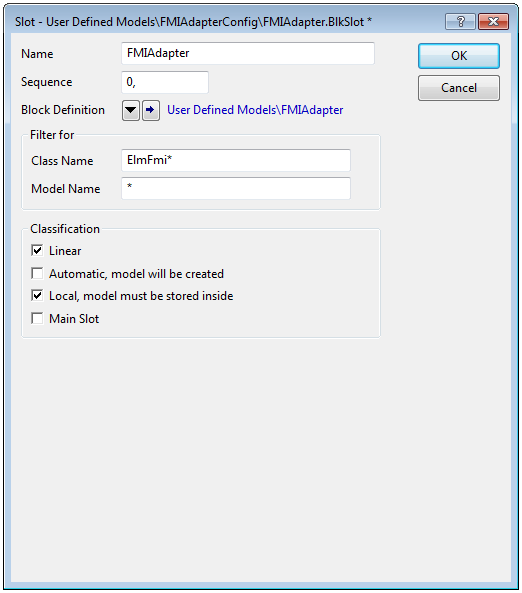
\includegraphics[width=0.6\textwidth]{fmiadapter_slot}}
\caption{Example of slot definition for \dslmodel FMIAdapter.}
\label{fig:fmiadapter_slot}
\end{figure}

\clearpage

\begin{figure}[h!]
\vspace*{2em}
\centering{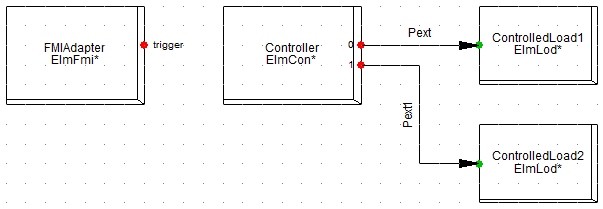
\includegraphics[width=0.9\textwidth]{fmiadapterconfig_composite_frame}}
\caption{Example of a composite frame including \dslmodel FMIAdapter.}
\label{fig:fmiadapterconfig_composite_frame}
\end{figure}


\subsection{Exporting an FMU from a model for RMS simulation}

\subsubsection*{Using the graphical user interface}

Once a \pf model according to the instructions above has been created, an FMU can be created with the help of the graphical user interface.
Switch to the installation directory and start program \texttt{powerfactory\_fmu\_install.exe} (double-click).
This should bring up the window shown in Figure~\ref{fig:gui_create}, where you can provide the following inputs:

\textit{Required arguments}:
\begin{itemize}
   \item \textbf{FMI model identifier}: Specify the FMU model identifier. 
   \emph{Attention}: The FMU model identifier must fulfill the restrictions for C function names!
   \item \textbf{\pf PFD file:} Export the \pf model as PFD file and provide its path (absolute or relative).
\end{itemize}

\textit{Time Advance Mechanism}:
\begin{itemize}
   \item \textbf{RMS simulation}:
   Specify the integrator step size in seconds.
   \item Leave the other boxes in this section empty.
\end{itemize}

\textit{Optional arguments}:
\begin{itemize}
   \item \textbf{Verbosity}: Turn on log messages.
   \item \textbf{Litter}: Do not clean-up intermediate files (e.g., log file with debug messages from Visual Studio compiler).
   \ietm \textbf{Input variable definition file} and \textbf{Output variable definition file}:
   Define which model variables of the \pf model should be exposed as input and output variables of the FMU.
   To do so, provide files containing lists of these variable names.
   These lists are expected to be in clear text, listing exactly one valid variable name per line.
   As explained in Section~\ref{sec:naming_convention:obj_param}, variable names are supposed to be of the  form \texttt{<obj-type>.<obj-name>.<param-name>}.
   \item \textbf{FMI version}: Specify FMI version (default: 2).
   \item \textbf{\pf installation directory}: Absolute path to \pf installation directory.\footnote{It is usually not necessary to provide the path to the \pf installation directory, unless the FMU is intended to run on another machine with a different installation directory path.}
   \item \textbf{Additional arguments}:
   \begin{itemize}
      \item Additional files may be specified (e.g., weather data or input/output name lists) that will be automatically copied to the FMU. The specified files paths may be absolute or relative.
      \item Start values for variables may be defined. For instance, to set variable with name \verb!var1! to value 12.34, specify \verb!var1=12.34! as optional argument.
   \end{itemize}
\end{itemize}


\subsubsection*{Export via Python script}

Alternatively, a \python script can be executed from the command prompt window (please refer to the \href{https://docs.python.org/3/faq/windows.html}{\python~FAQ} in case you need assistance with this).
Open the command prompt window and execute the script \texttt{powerfactory\_fmu\_create.py}:

\begin{verbatim}
python.exe <path_to_pf_fmu_dir>powerfactory_fmu_create.py [-h] [-v] 
  [-f {1,2}] -m model_id -p pfd_file -i input_var_file 
  -o output_var_file -r step-size [-d pf_install_dir] 
  [additional_file_1 ... ] [var1=start_val1 ...]
\end{verbatim}

The path to the \fmipp \pf FMU export utility directory \verb!<path_to_pf_fmu_dir>! may be relative or absolute.
Optional arguments are enclosed by squared brackets \verb![!$\,$\ldots\verb!]!.
  
\textit{Mandatory input arguments}:
\begin{itemize}
  \item \verb!-m, --model-id!: specify FMU model identifier
  \item \verb!-p, --pfd-file!: path to PowerFactory PFD file
  \item \verb!-i, --input-var-file!: specify file containing list of input variable names
  \item \verb!-o, --output-var-file!: specify file containing list of output variable names
  \item \verb!-r, --rms-sim!: specify the integrator step size in seconds
\end{itemize}
\textit{Optional input arguments}:
\begin{itemize}
  \item \verb!-f, --fmi-version!: specify the FMI version (1: FMI~1.0, 2: FMI~2.0, default: 2)
  \item \verb!-h, --help!: display the help screen
  \item \verb!-v, --verbose!: turn on log messages
  \item \verb!-l, --litter!: do not clean-up intermediate files
  \item \verb!-d, --pf-install-dir!: path to \pf installation directory\footnote{It is usually not necessary to provide the path to the \pf installation directory, unless the FMU is intended to run on another machine with a different installation directory path.}
\end{itemize}
Files containing lists of input and output variable names are expected to be in clear text, listing exactly one valid variable name per line.
As explained in Section~\ref{sec:naming_convention}, variable names are supposed to be of the form \texttt{EvtParam.<slot-name>.<param-name>} (for input simulation events) or \texttt{<obj-type>.<obj-name>.<param-name>} (for output object parameters).

Additional files may be specified that will be automatically copied to the FMU. The specified files paths may be absolute or relative.

Furthermore, start values for variables may be defined (referring to object parameters and simulation events). For instance, to set a variable with the name \texttt{ElmLod.TestLoad.plini} to a value of 12.34, specify \texttt{ElmLod.TestLoad.plini=12.34} in the command line as optional argument.

Section~\ref{sec:examples:rmssim} gives a concrete example of how to export a model for RMS simulation as an FMU.

